\setAuthor{Jaan Kalda}
\setRound{piirkonnavoor}
\setYear{2007}
\setNumber{G 2}
\setDifficulty{1}
\setTopic{Kinemaatika}

\prob{Ummik}
Vaatleme kahe üherajalise tee, $A$ ja $B$, liitumist üherajaliseks teeks $C$. Tipptunni ajal on kõik kolm teed täidetud autodega; kahe naaberauto keskmise vahemaa võib lugeda kõigil kolmel teel ühesuguseks. Tee $A$ pikkus on $L_A = \SI{1}{km}$, tee $B$ pikkus $L_B = \SI{3}{km}$ ning tee $C$ pikkus $L_C = \SI{2}{km}$. Autode keskmine kiirus teel $A$ on $v_A = \SI{3}{km/h}$ ning tee $B$ läbimiseks kulub autol $t_B = \SI{36}{min}$. Kui kaua kulub autol jõudmaks tee $A$ algusest tee $C$ lõpuni?
\begin{center}
	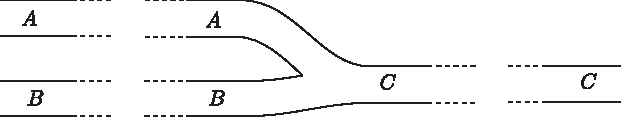
\includegraphics[width=0.9\linewidth]{2007-v2g-02-yl}
\end{center}

\hint
Autode hulga pidevuse tõttu on lõigul $C$ teatud punkti ajaühikus läbivate autode arv võrdne lõikude $A$ ja $B$ vastavate arvude summaga.

\solu
Lõigul $C$ on teatud punkti ajaühikus läbivate autode arv $N_C$ võrdne lõikude $A$ ja $B$ vastavate arvude summaga: $N_C = N_A + N_B$. Olgu autode vahemaa $a$ ja vaadeldav ajavahemik $\tau$. Siis $N_i = v_i\tau /l$, ehk 
\[
\frac{v_{C} \tau}{l}=\frac{v_{A} \tau}{l}+\frac{v_{B} \tau}{l} \quad \Rightarrow \quad v_{C}=v_{A}+v_{B}.
\]
Et $v_B = L_B/t_B$, siis toodud arvude põhjal leiame 
\[
v_{B}=\frac{\SI{3}{km}}{\SI{36}{min}}=\SI{5}{km/h}
\]
ning seega $v_C = \SI{8}{km/h}$. Lõpetuseks, $t_A = L_A/v_A=\SI{20}{min}$ ja $t_C = L_C/v_ = \SI{15}{min}C$. Niisiis kulub autol aega $T = t_A + t_C = \SI{35}{min}$.
\probend